\pagenumbering{roman}
\setcounter{page}{1}

\section*{Appendix}
\label{sec:appendix}

\setcounter{subsection}{0}
\renewcommand{\thesubsection}{\Alph{subsection}}

\subsection{Cluster Profiles}

Many more quantities and modifications could be added to the previously defined radial profiles.
Noting an interesting consequence of the self similarity between galaxy clusters, different
characteristic overdensity averages are determined by $R_\ell$ and $M_\ell$ alone. Accordinly,
combining values listed in \Cref{tab:obs_param} allows us to estimate averages for $T_\ell$ as
well as $P_\ell$ and $K_\ell$ where in addition we must only account for the simplified
cosmological evolution parameter
\begin{equation*}
	h(z) = \frac{H(z)}{H_0} = \sqrt{\Omega_M(1 \kern-1pt+\kern-0.5pt z)^3 + \Omega_{\kern-1pt\Lambda}}
\end{equation*}
under the condition $\Omega_M + \Omega_\Lambda = 1$ for a flat universe. Exact equations based on the
REXCESS sample among others are given in the literature \cite{arna2005, arna2010, prat2010}.


\begin{figure*}
	\centering
	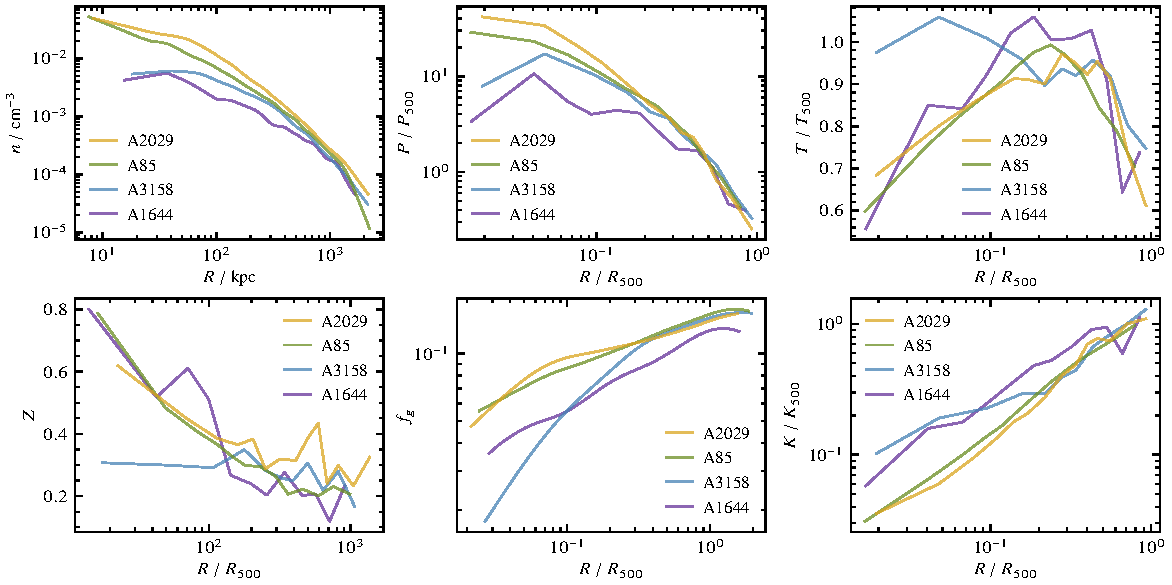
\includegraphics[width=\textwidth, draft=false]{content/xmmn_profiles.pdf}
	\caption{Plots of extracted radial profile projections for available \textit{X{\hspace{0.04em}\dash\hspace{0.11em}}COP}
			 galaxy clusters. \textit{Upper Left:} Electron number density. \textit{Upper Middle:} Gas pressure.
			 \textit{Upper Right:} Gas temperature. \textit{Lower Right:} Gas entropy. \textit{Lower Middle:}
			 Gas mass fraction. \textit{Lower Left:} Metal abundance. Consult the text for definitions of characteristic
			 quantities and scaling. Compare as well to reconstructed distributions in \Cref{fig:chan_profiles} which
			 focus on the inner regions instead of the cluster outskirts.}
	\label{fig:xmmn_profiles}
\end{figure*}

\subsection{Reference Images}

To supplement the composites in \Cref{fig:obs_overlay} with intermediate pipeline data, \Cref{fig:obs_raw} displays the
raw count rates after an initial smoothing.


\begin{figure*}
	\centering
	\begin{subfigure}[b]{0.33\textwidth}
		\centering
		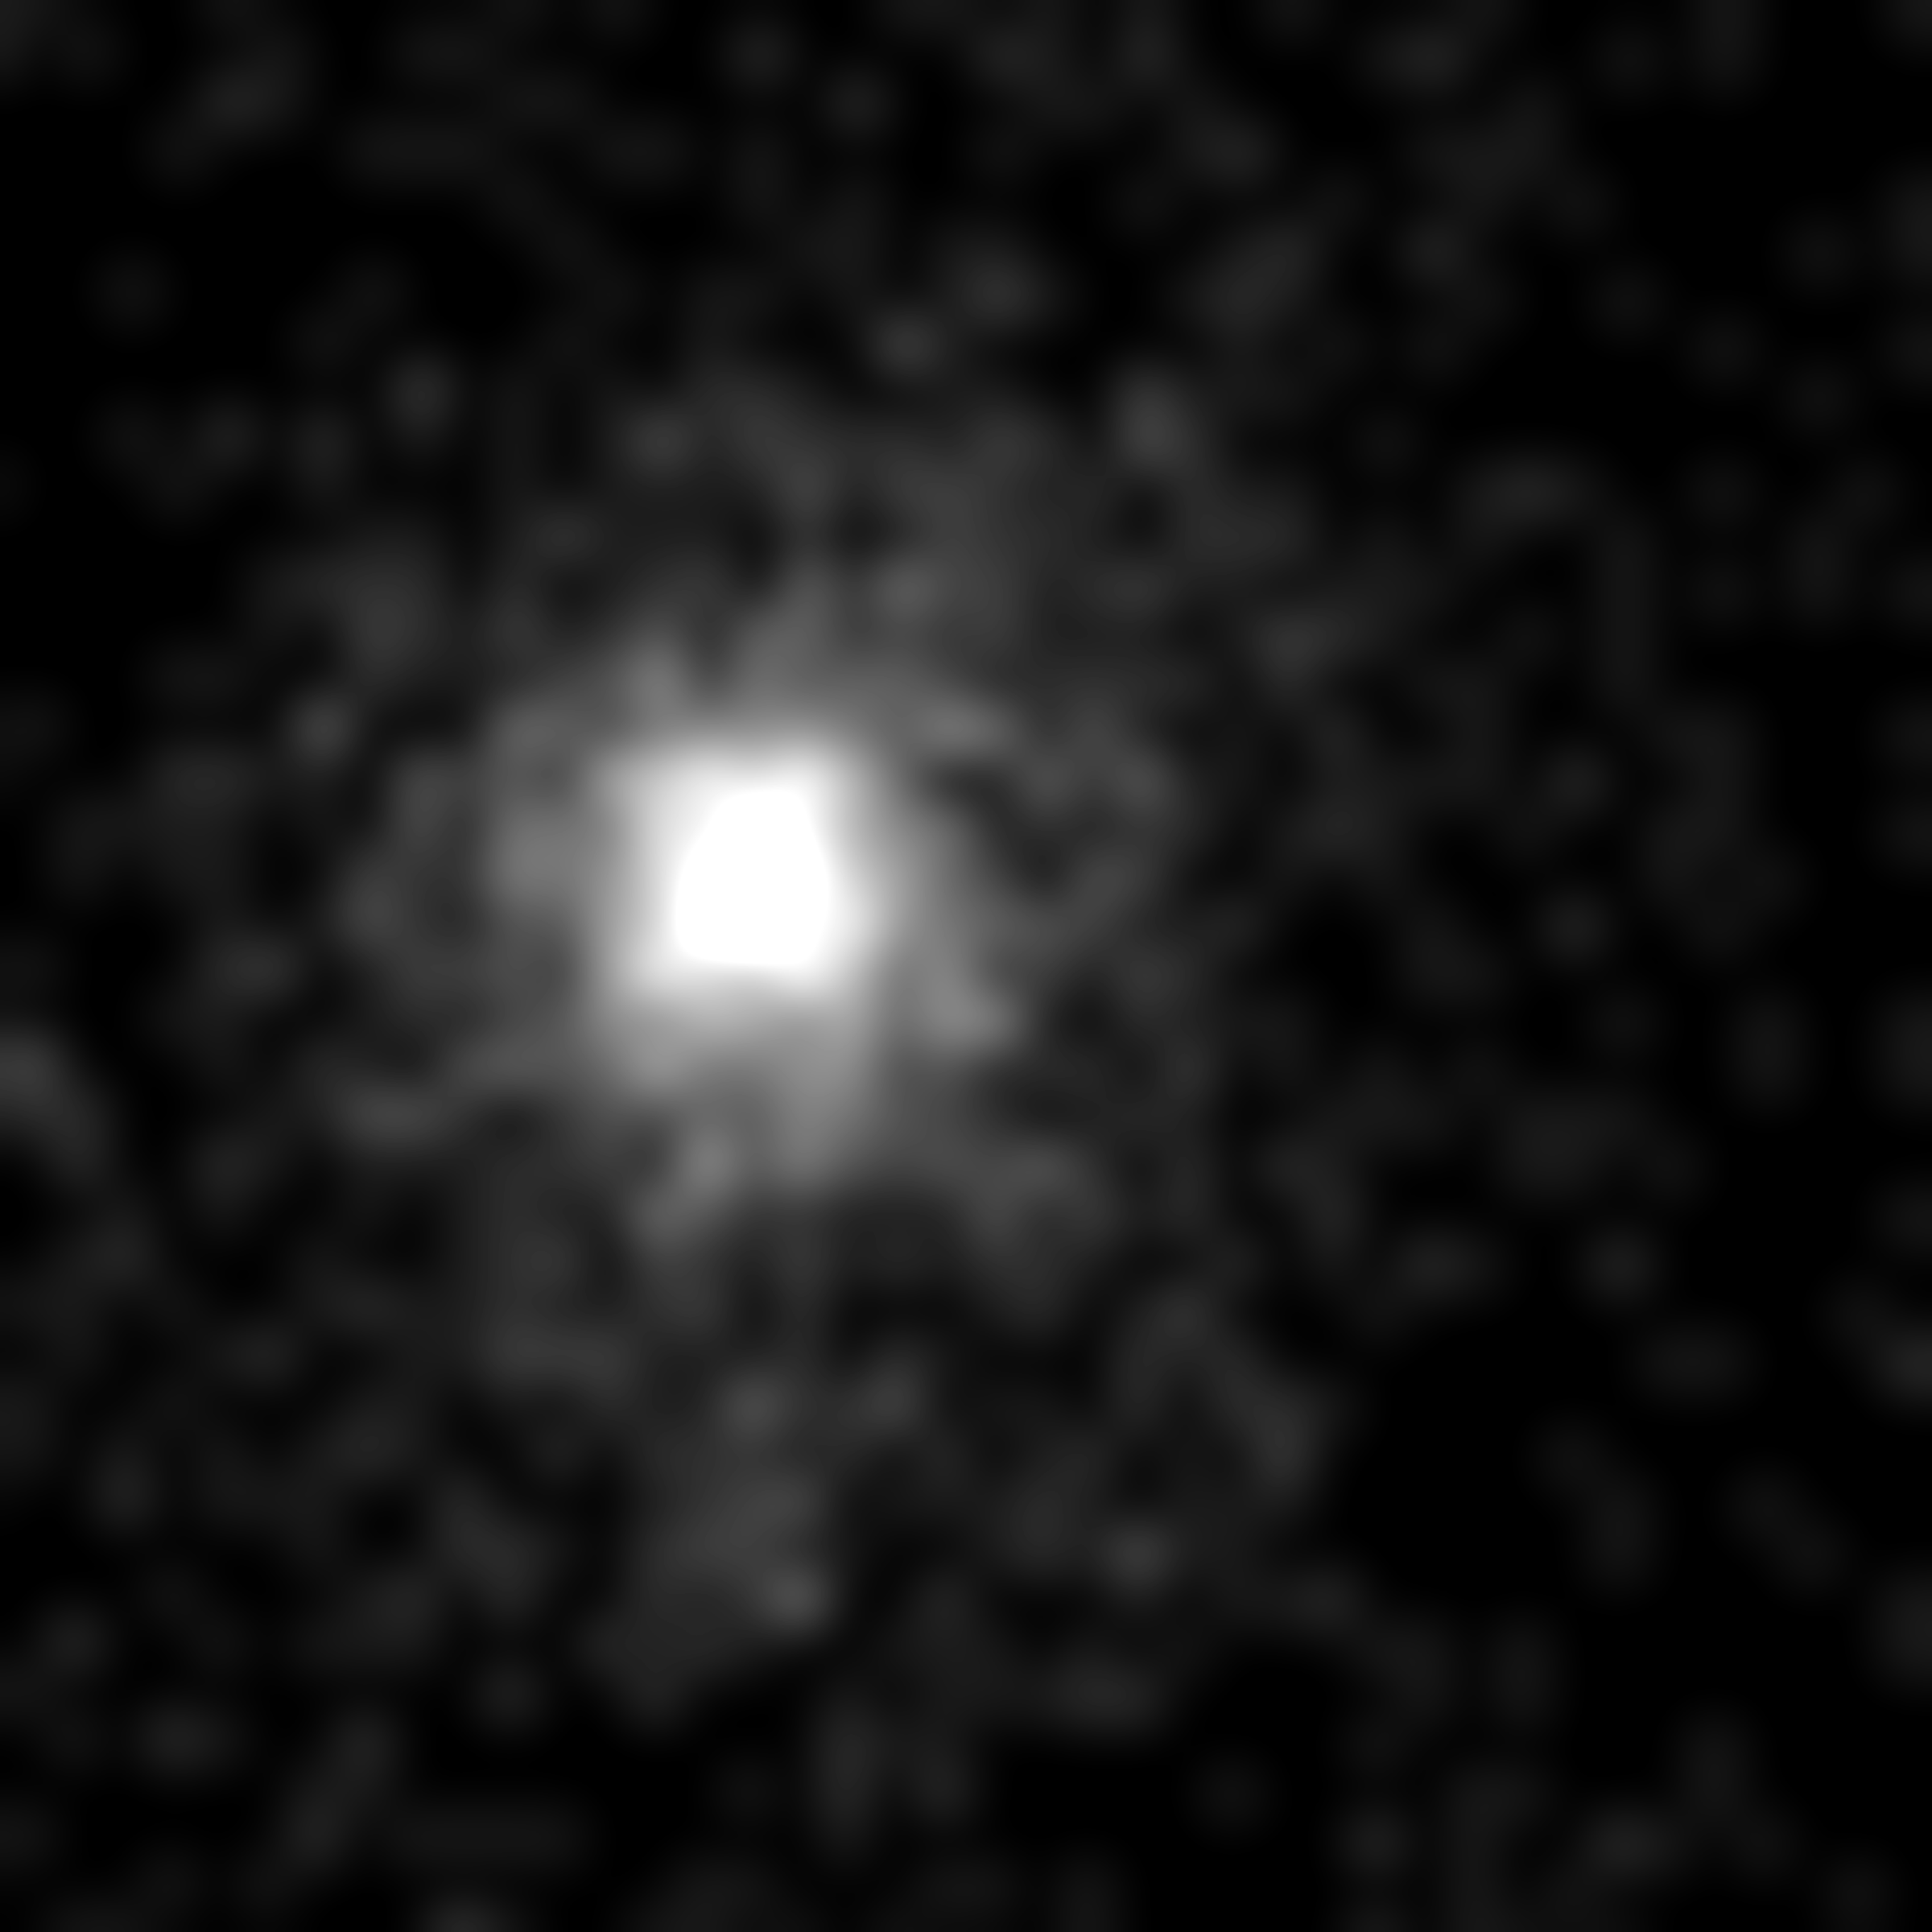
\includegraphics[width=\textwidth]{catalog/ROSAT/RASS-DSS2-A85-raw.png}
		\caption{Abell 85}
	\end{subfigure}
	\hfill
	\begin{subfigure}[b]{0.33\textwidth}
		\centering
		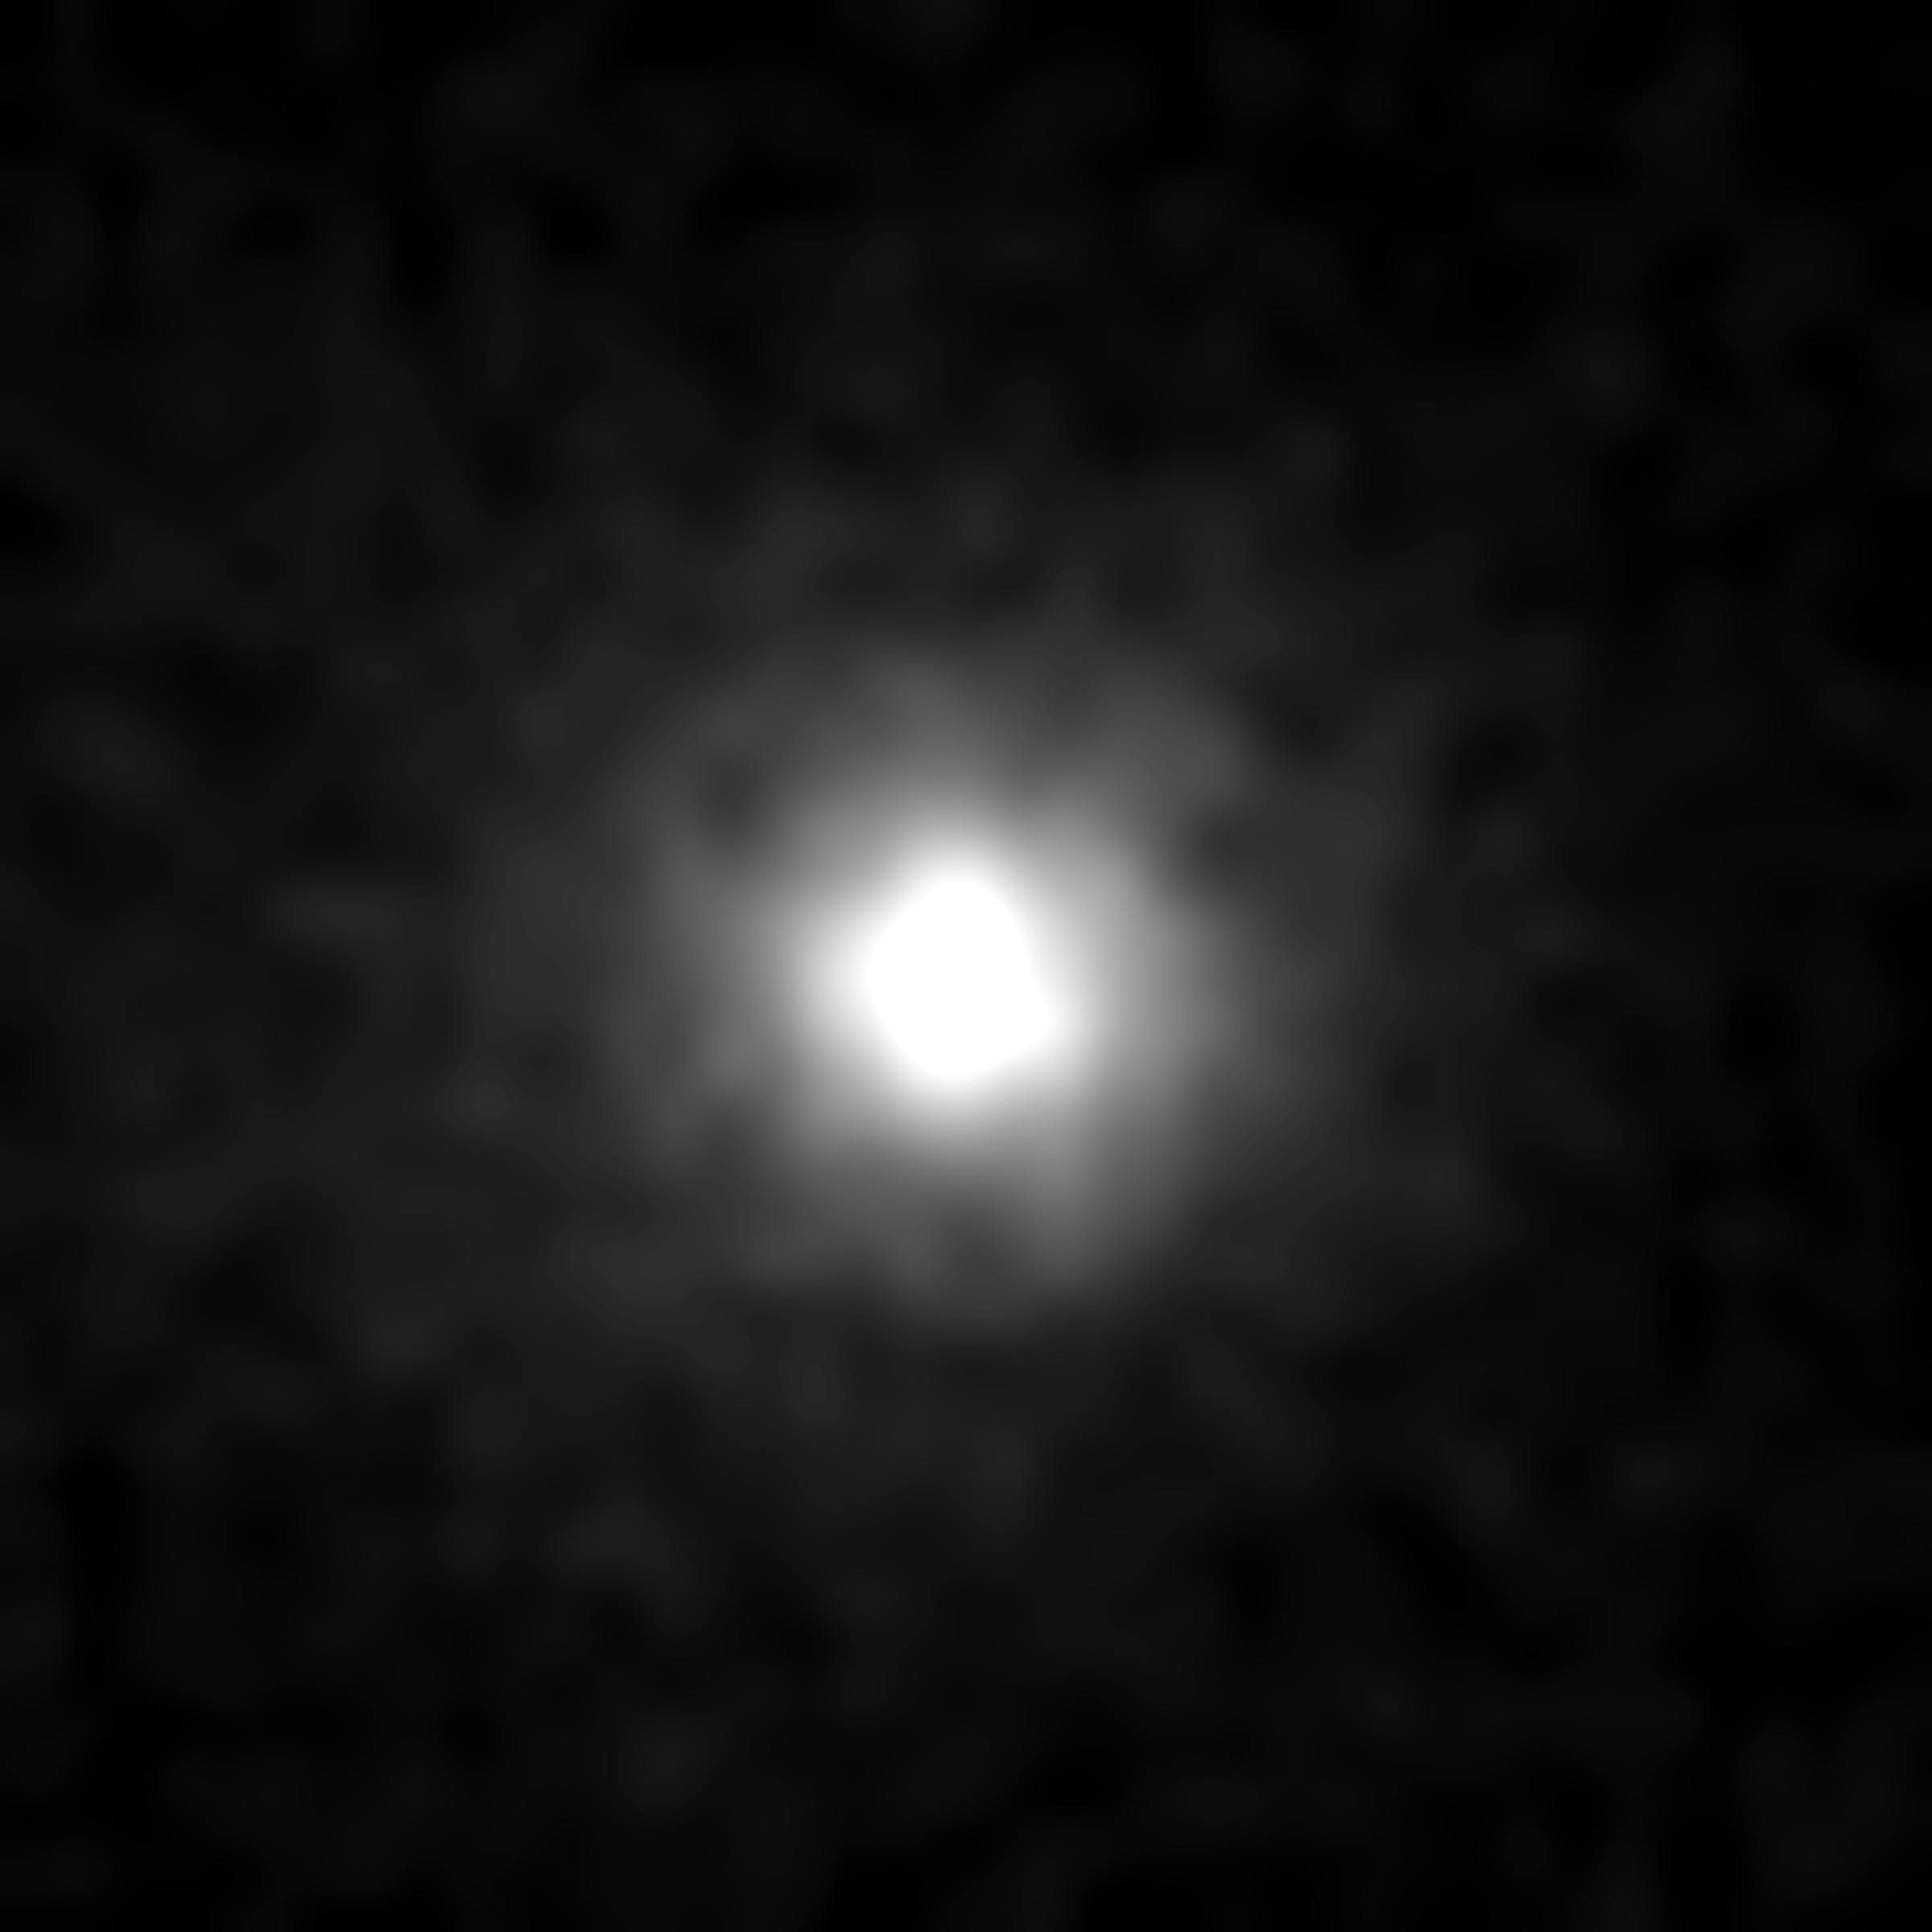
\includegraphics[width=\textwidth]{catalog/ROSAT/RASS-DSS2-A426-raw.png}
		\caption{Abell 426 (Perseus)}
	\end{subfigure}
	\hfill
	\begin{subfigure}[b]{0.33\textwidth}
		\centering
		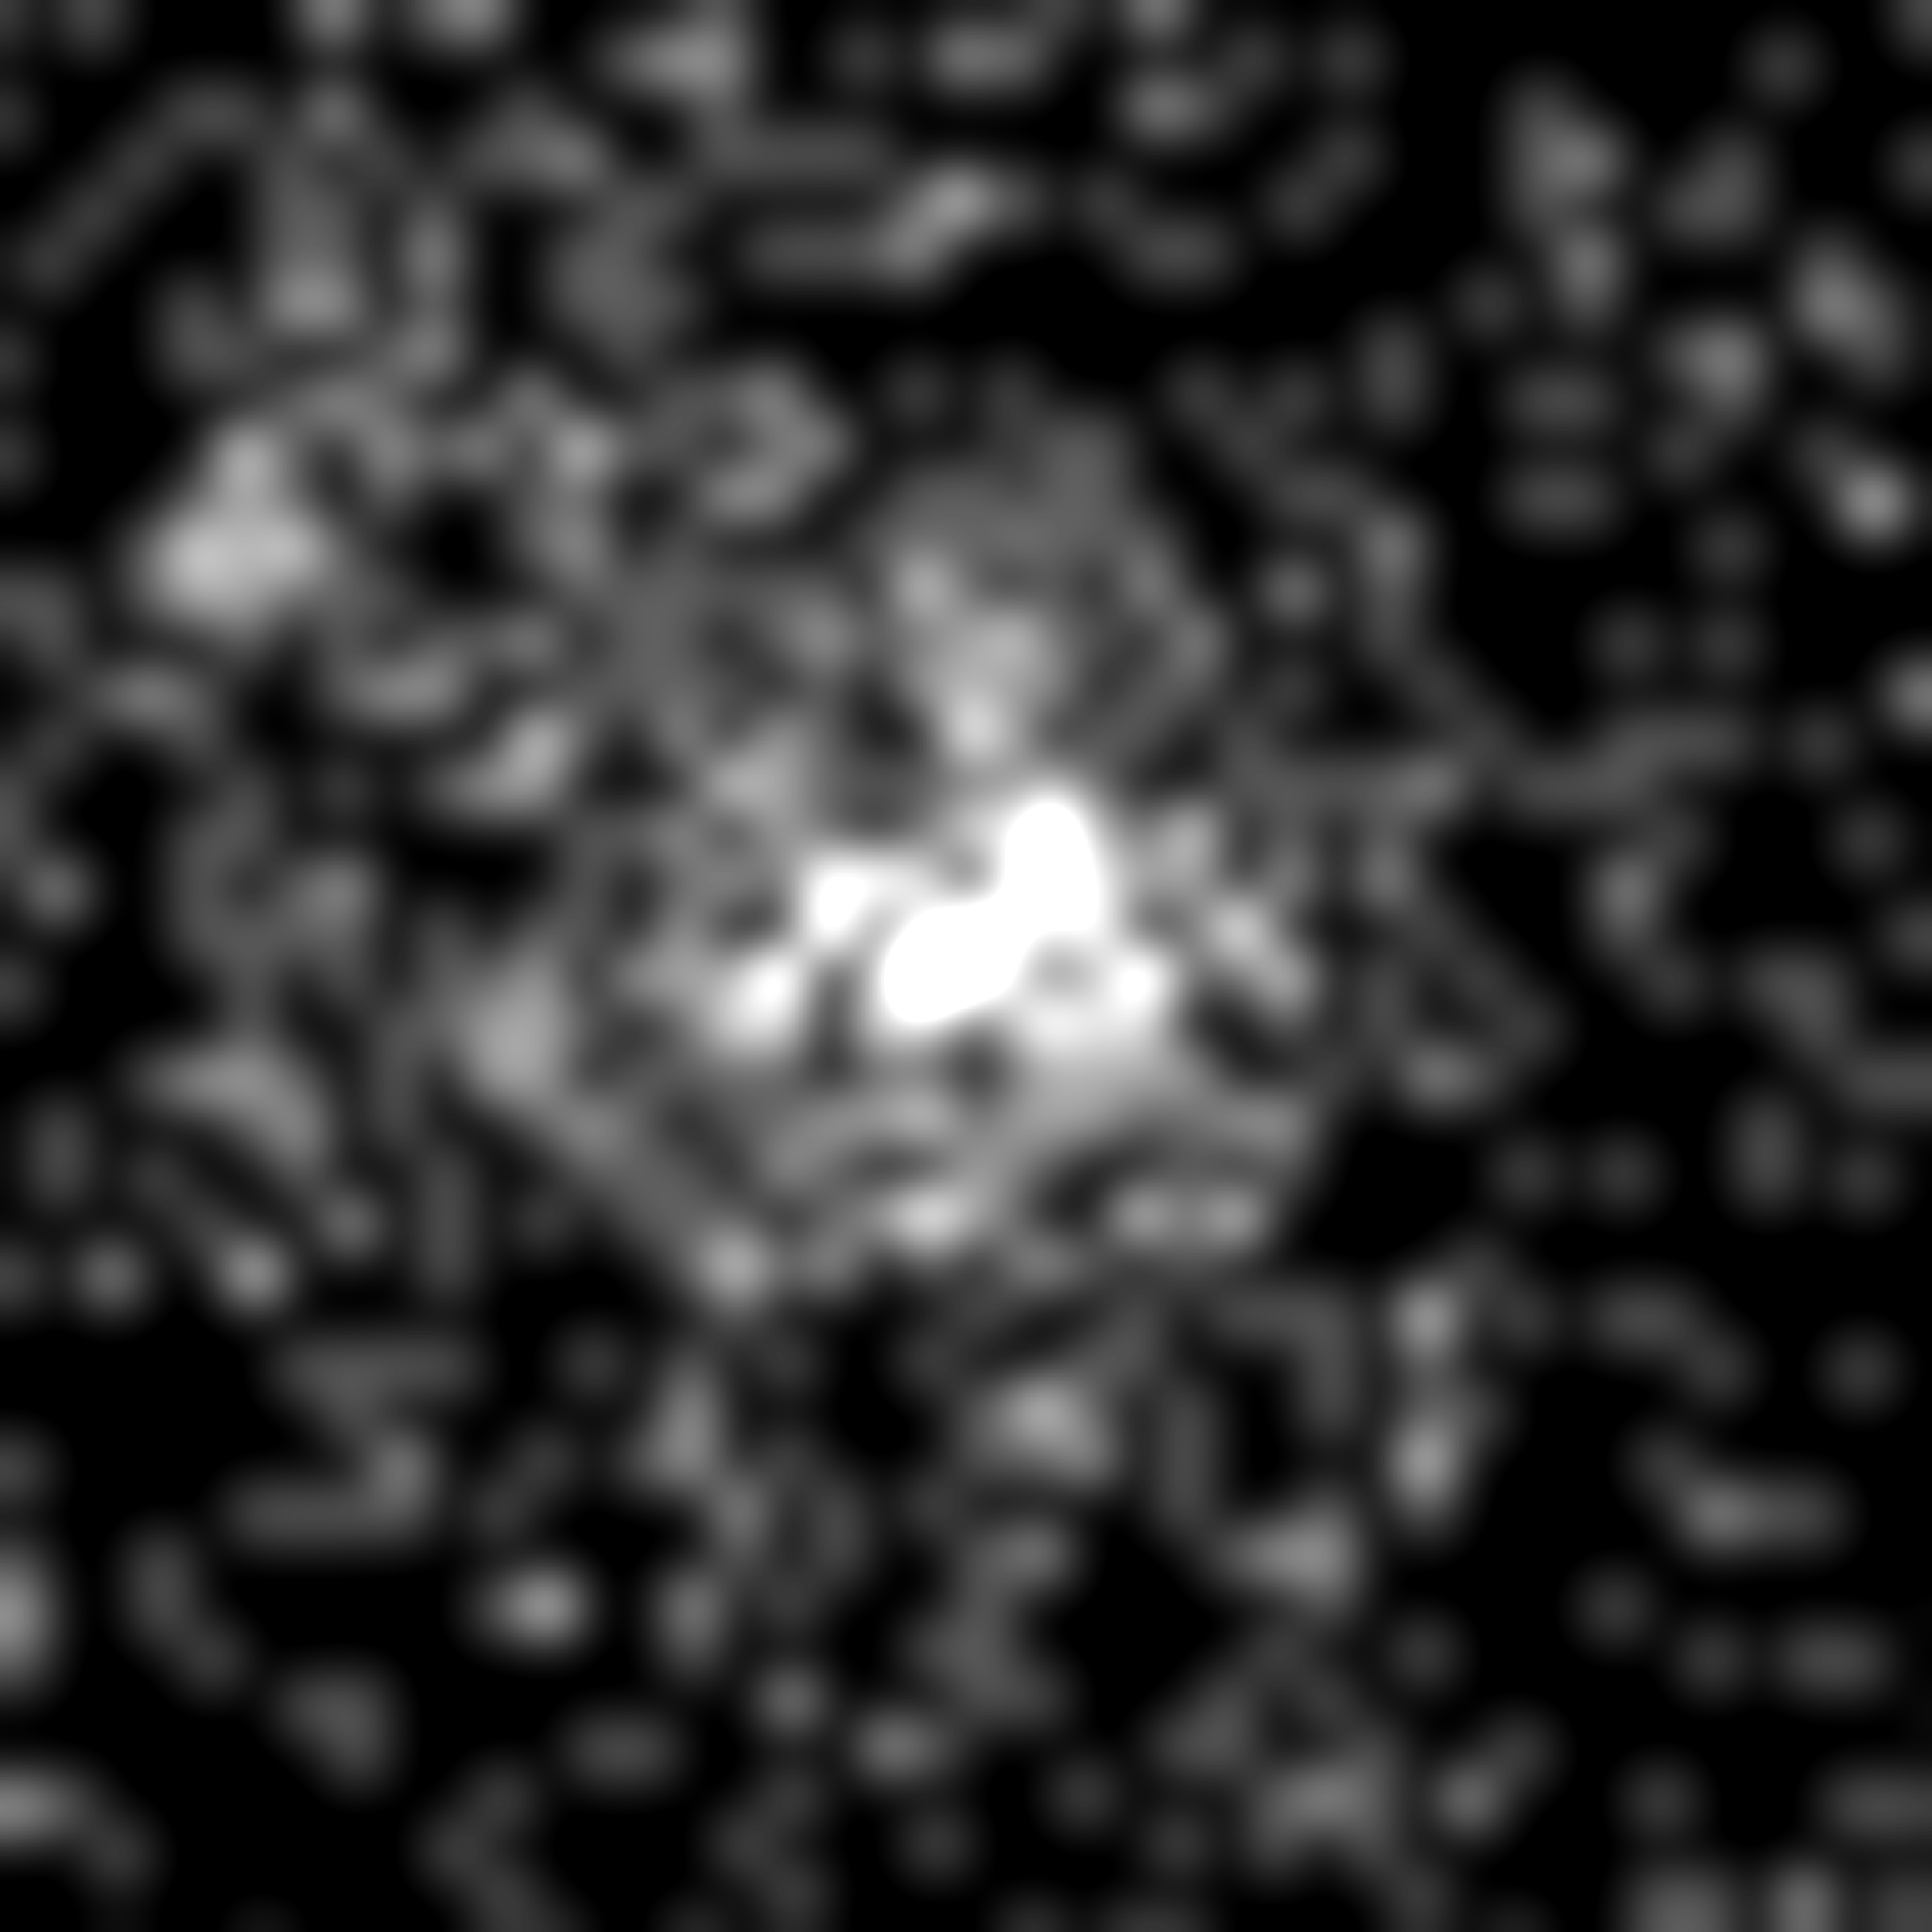
\includegraphics[width=\textwidth]{catalog/ROSAT/RASS-DSS2-A1644-raw.png}
		\caption{Abell 1644}
	\end{subfigure}

	\vspace{1ex}

	\begin{subfigure}[b]{0.33\textwidth}
		\centering
		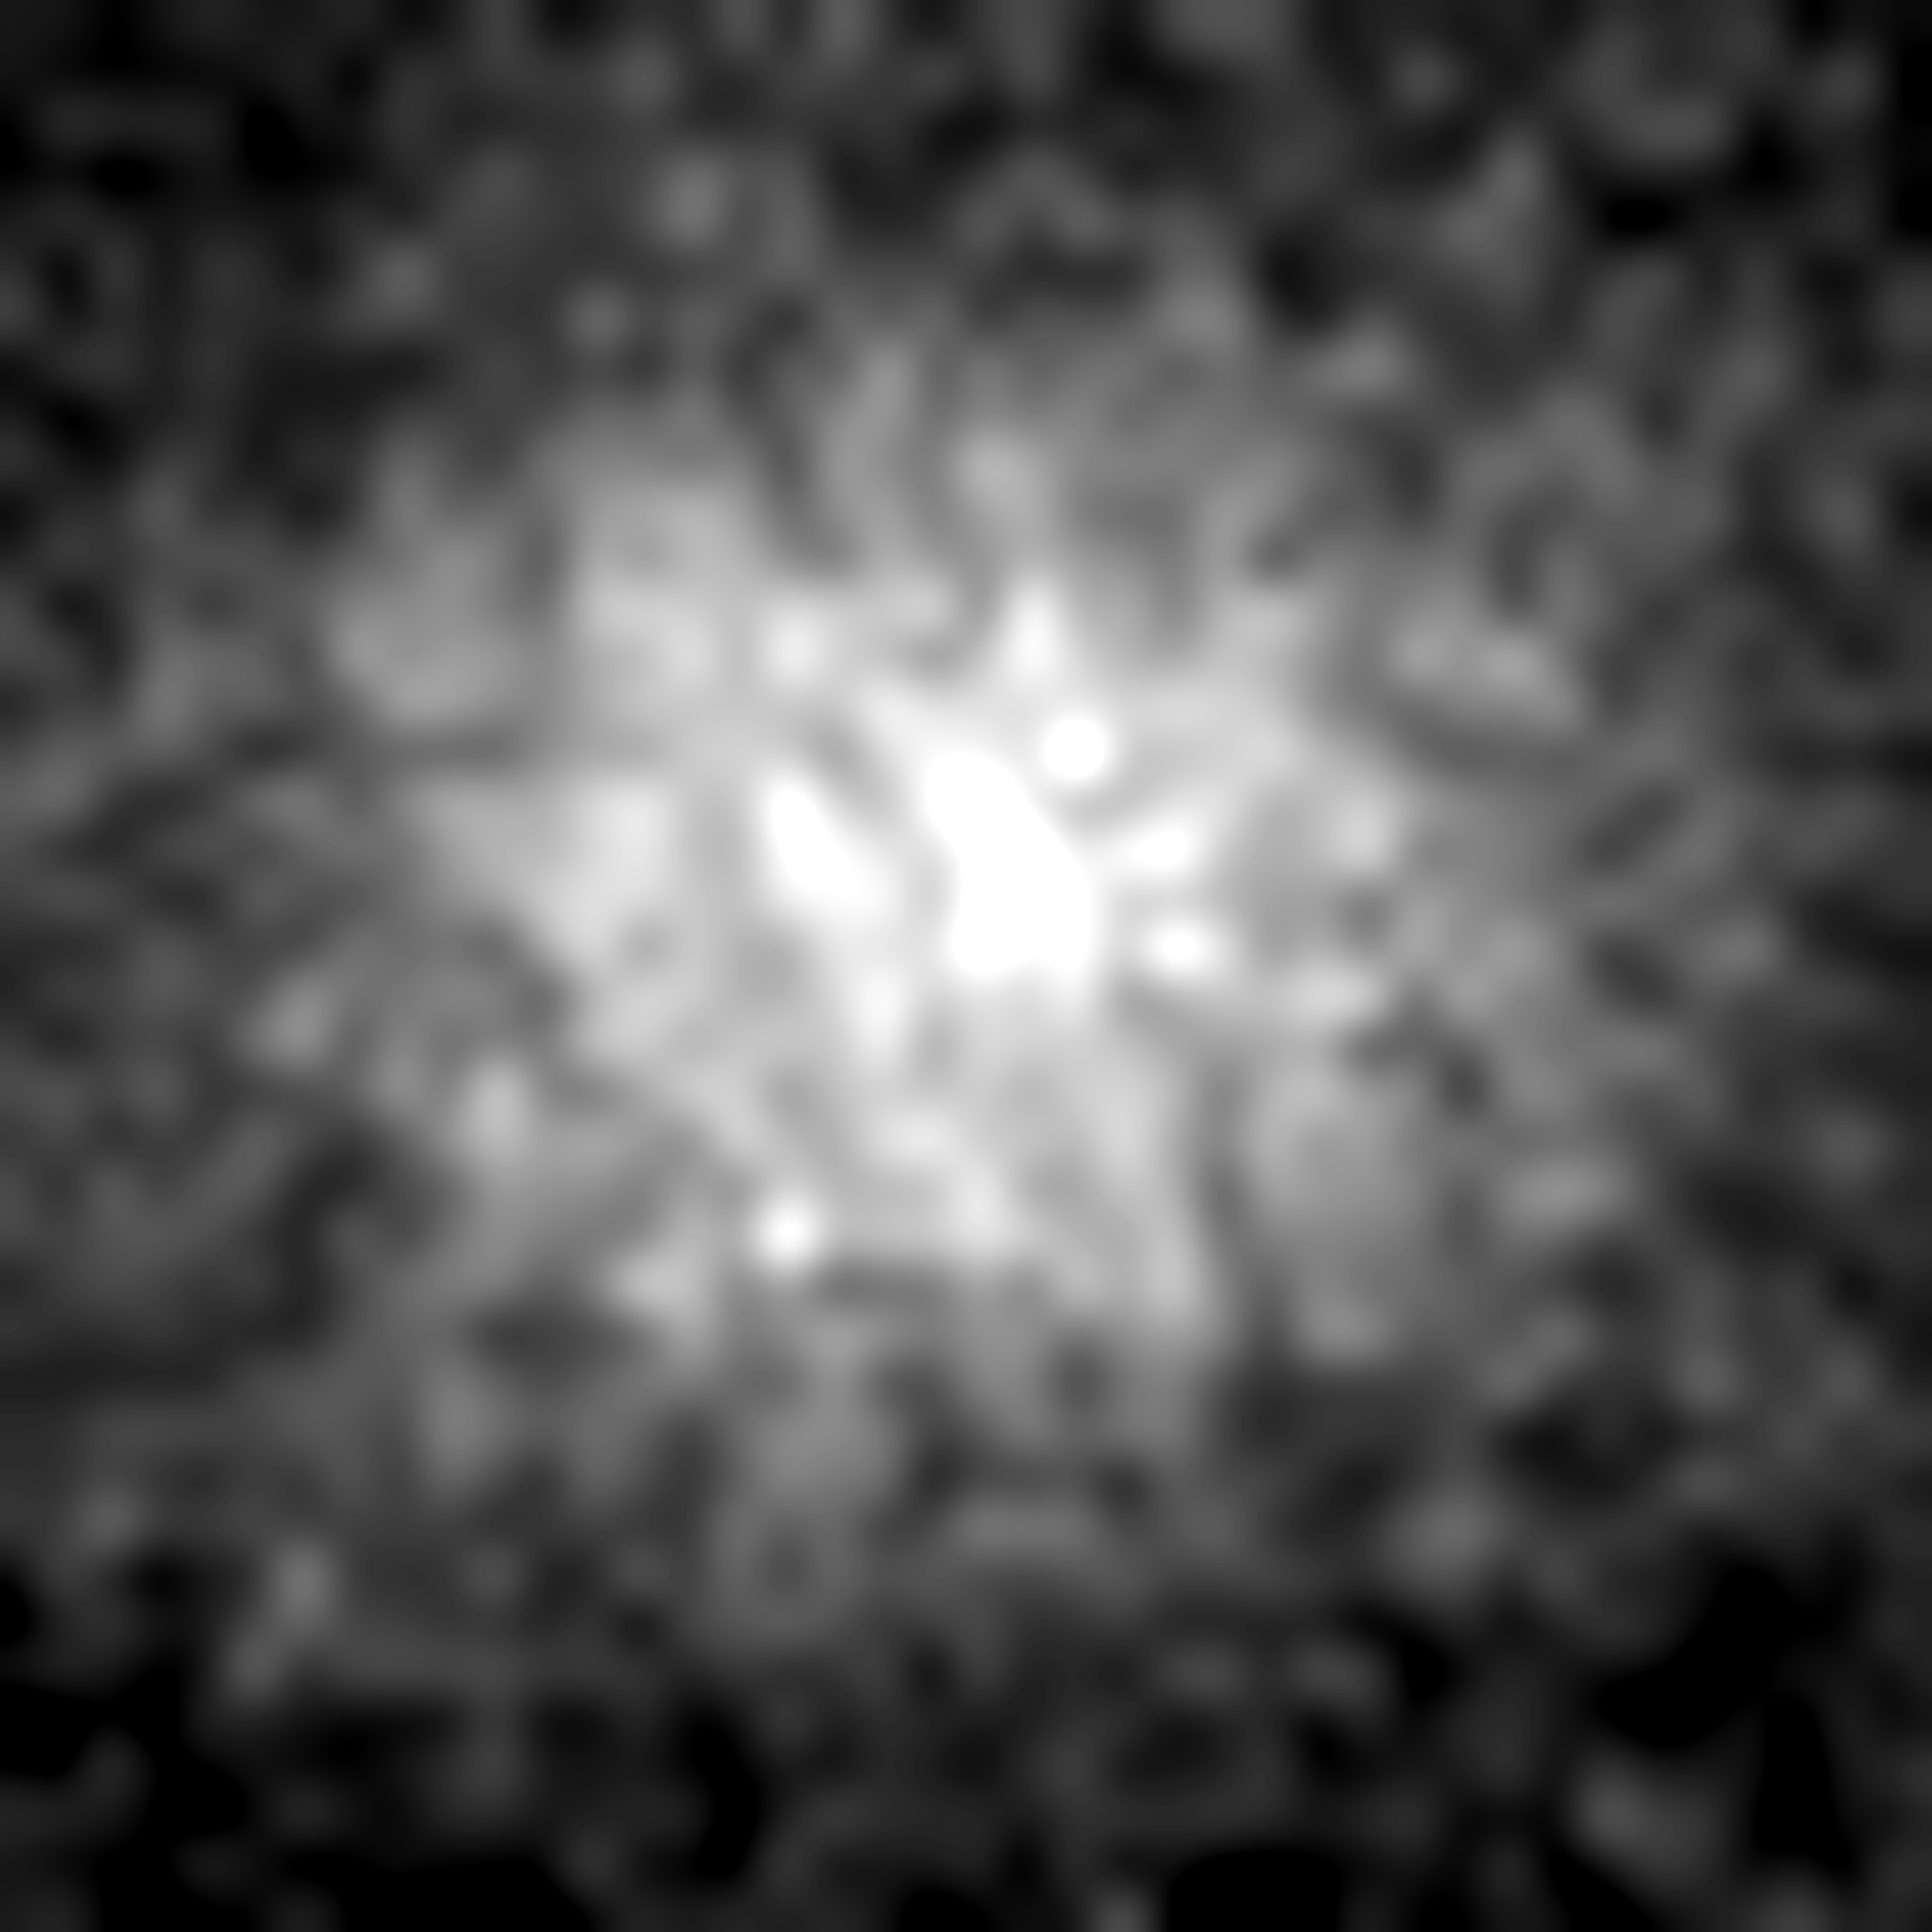
\includegraphics[width=\textwidth]{catalog/ROSAT/RASS-DSS2-A1656-raw.png}
		\caption{Abell 1656 (Coma)}
	\end{subfigure}
	\hfill
	\begin{subfigure}[b]{0.33\textwidth}
		\centering
		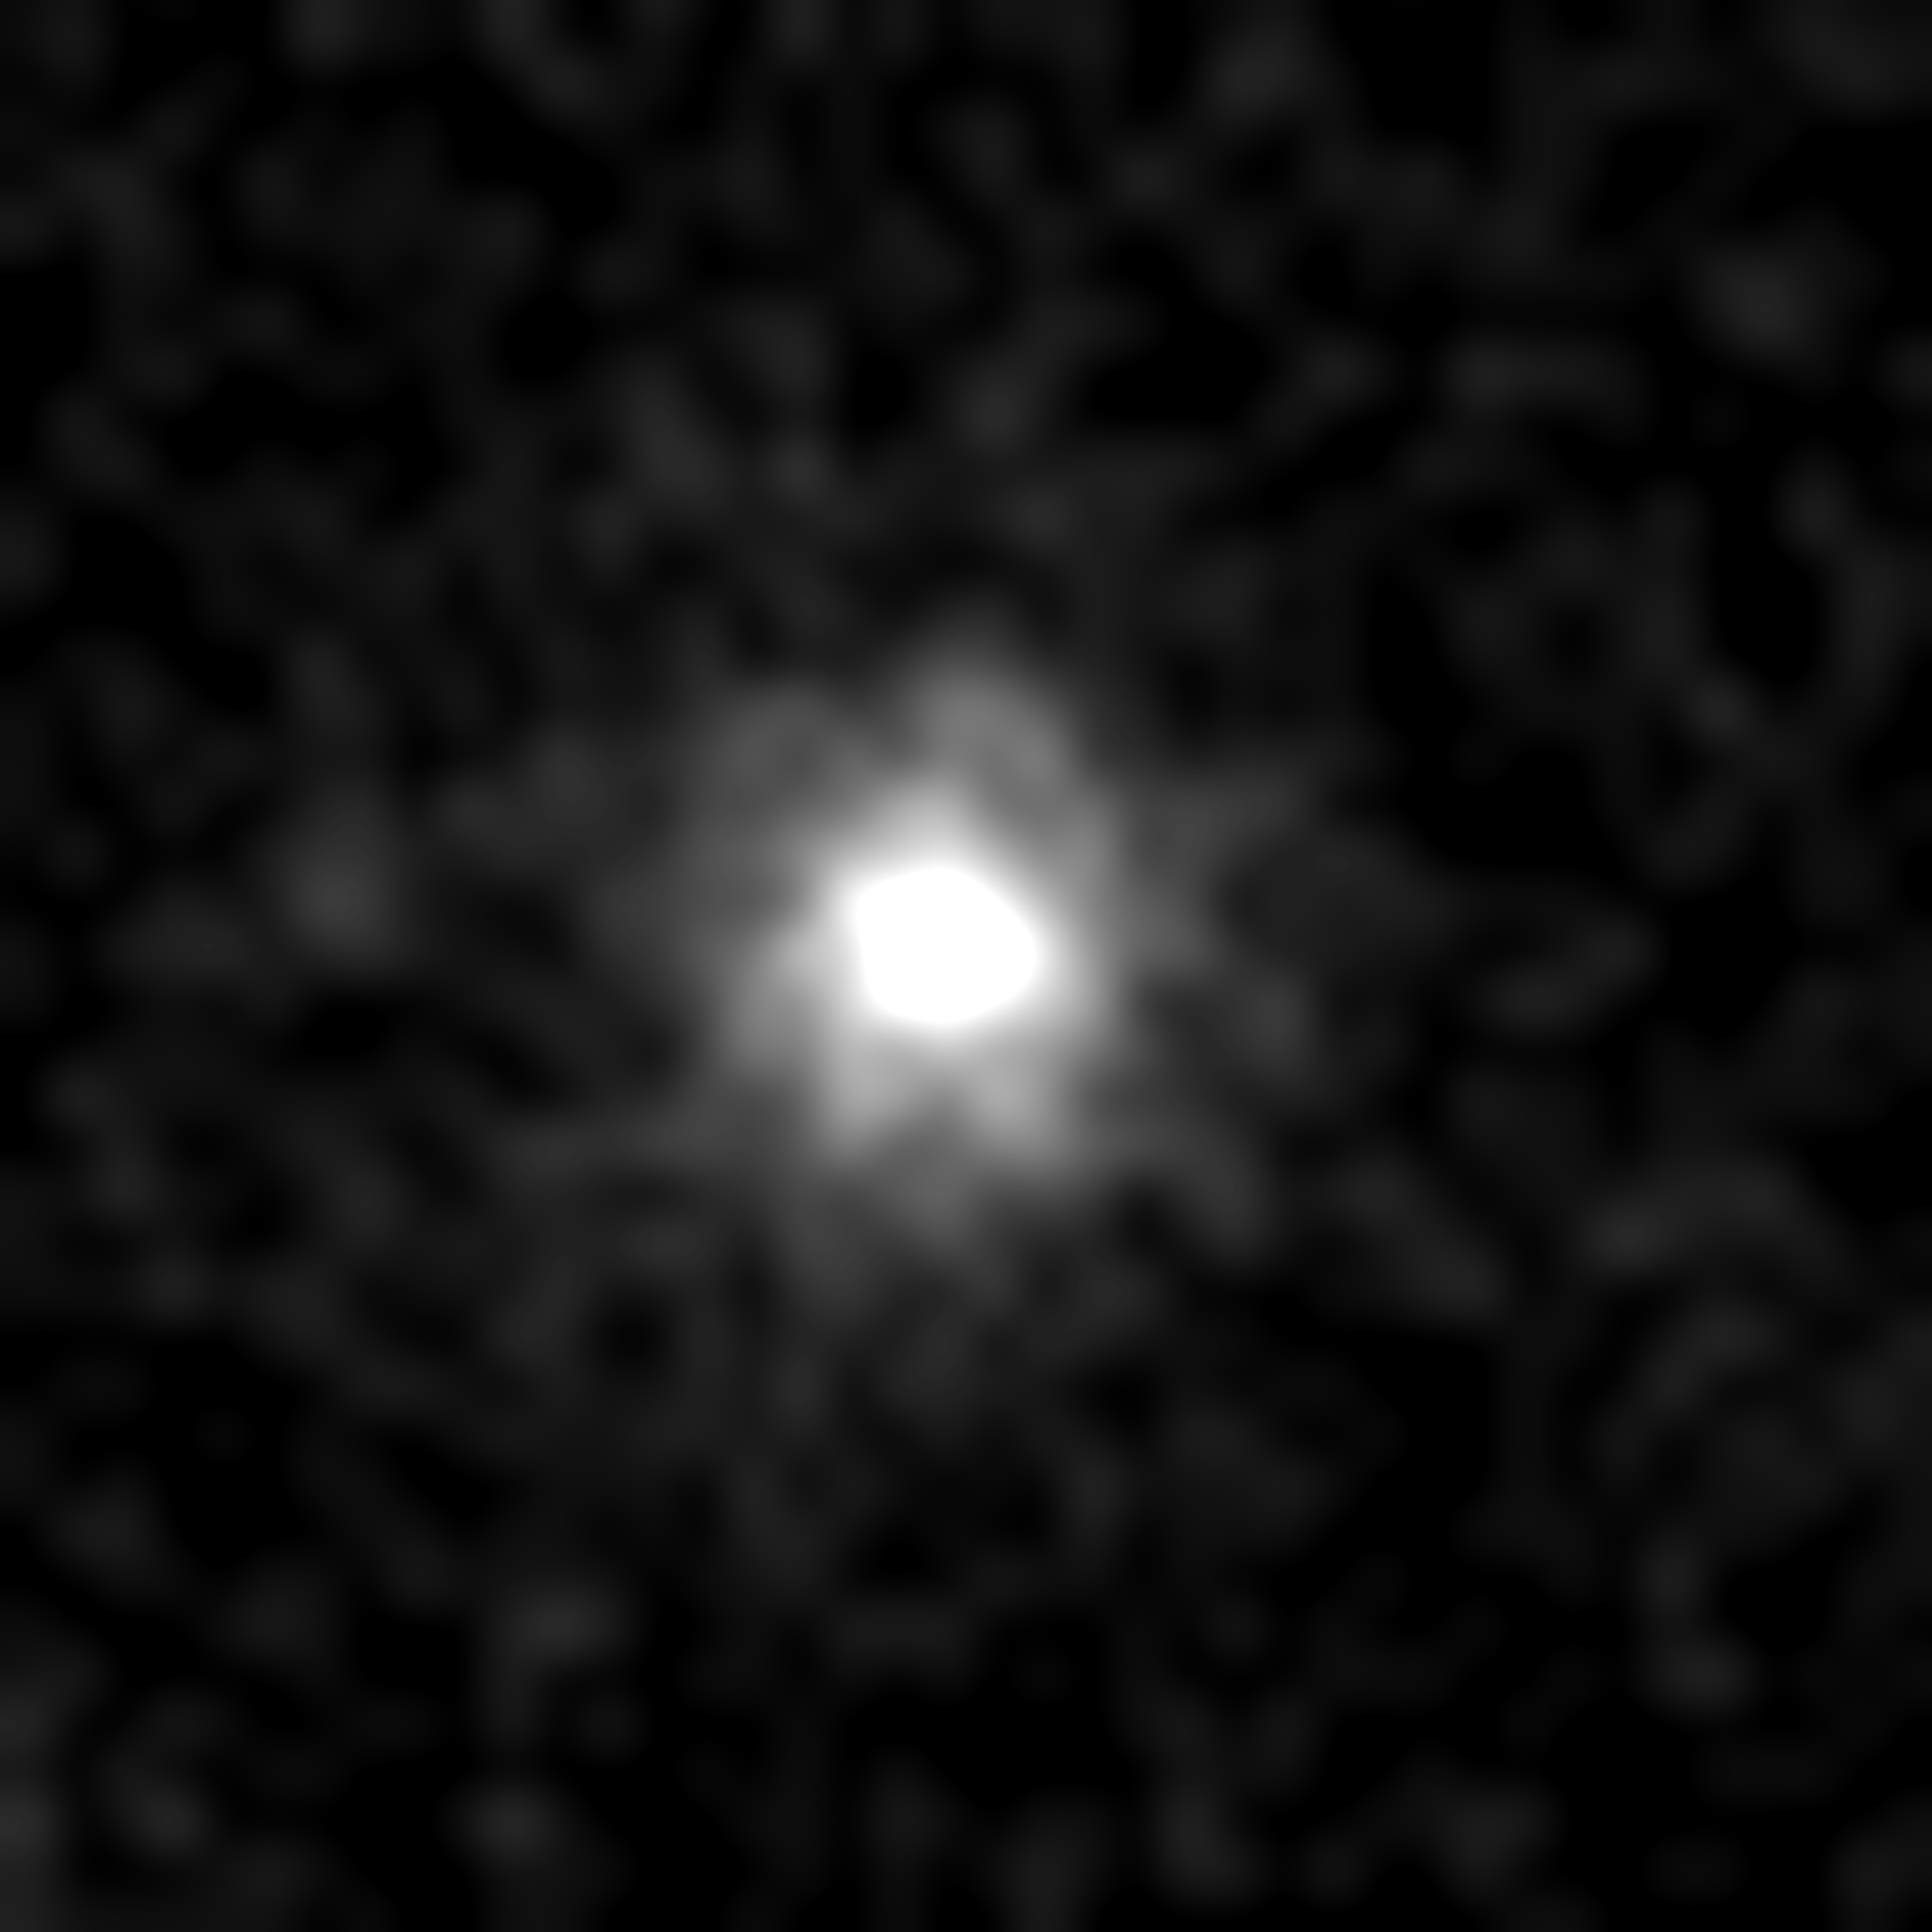
\includegraphics[width=\textwidth]{catalog/ROSAT/RASS-DSS2-A2029-raw.png}
		\caption{Abell 2029}
	\end{subfigure}
	\hfill
	\begin{subfigure}[b]{0.33\textwidth}
		\centering
		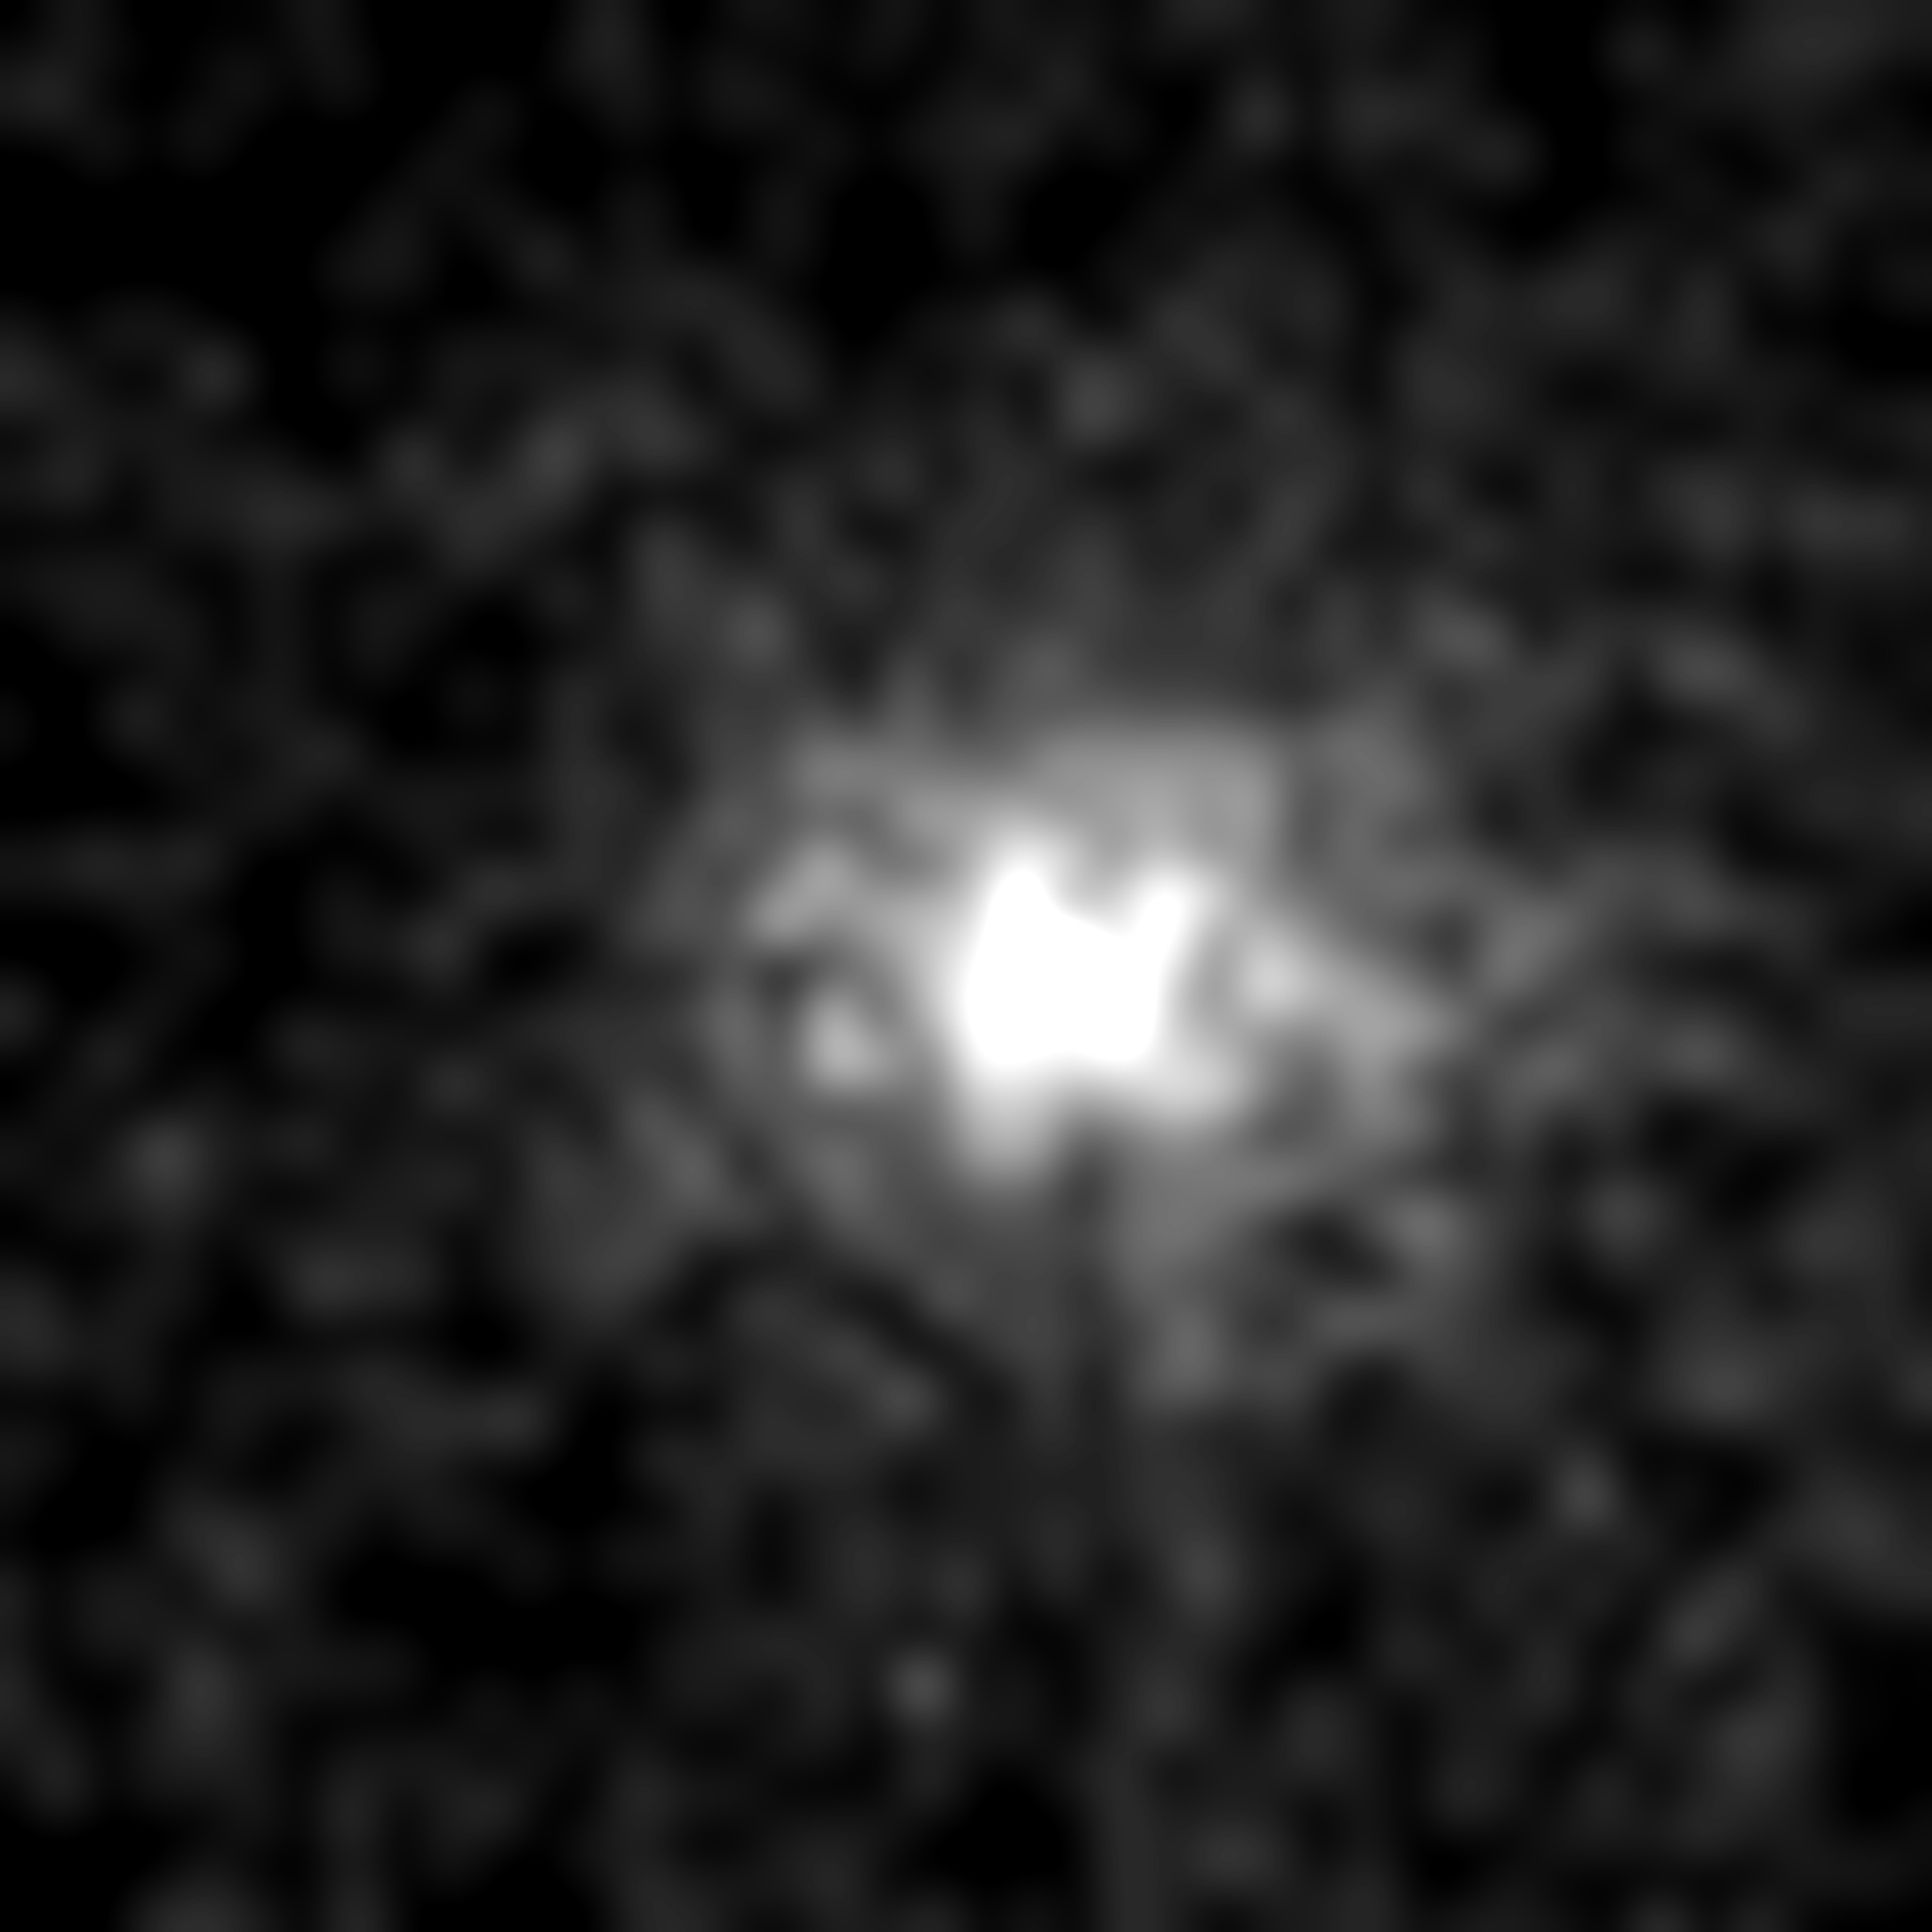
\includegraphics[width=\textwidth]{catalog/ROSAT/RASS-DSS2-A3158-raw.png}
		\caption{Abell 3158}
	\end{subfigure}
	\caption{Depicted are \textit{RASS} counts used for \xray contours shown in
			 \Cref{fig:obs_overlay} after applying a stretch and Gaussian blur \cite{true1982}.
			 The sampled clusters are selected based on brightness and morphology, as well
			 as data accessibility in the \textit{Archive of Chandra Cluster Entropy Profile
			 Tables (ACCEPT)} and \textit{XMM Cluster Outskirts Project (X{\hspace{0.04em}\dash\hspace{0.11em}}COP)}
			 catalogs \cite{cava2009, ecke2017}.}
	\label{fig:obs_raw}
\end{figure*}


\subsection{Methodology}

All figures included in this text are generated using a semi automated Python pipeline that
matches and pulls from the NASA High Energy Astrophysics Science Archive Research Center
(HEASARC) or SkyView databases, and extracts locally saved archival data files saved manually
directly from the different collaborations cited in this work. The relevant components
are then cleaned and processed to be ingested by the plotting script itself. To reproduce and modify the
implementation, consult this \href{https://github.com/fritzali/notes/tree/main/MASS/Spectroscopy}{repository}.
